\section{Исследовательский раздел}
\subsection{Предмет исследования}
В данной работе будут рассмотрены следующие зависимости:
\begin{itemize}[leftmargin=1.6\parindent]
	\item[--] зависимость времени работы метода от количества изображений;
	\item[--] зависимость точности модели нейронной сети от размера изображений.
\end{itemize}

Время работы метода напрямую зависит от количества изображений, подаваемых на вход, так как основной операцией является классификация изображения. Точность модели зависит в основном от размера (качества) изображений и ракурса, так как в наборе данных нет изображений под другим ракурсом, то будет рассмотрена зависимость от качества изображений.

\subsection*{Технические характеристики}
Технические характеристики устройства, на котором выполнялись сравнения, следующие.

\begin{itemize}
	\item[--] Операционная система: macOS 12.5.1.
	\item[--] Память: 32 ГБ.
	\item[--] Процессор: Apple M1 Pro CPU @ 3.22ГГц \cite{apple}.
\end{itemize}
Исследование проводилось на ноутбуке, включенном в сеть электропитания. Во время экспериментов ноутбук был нагружен только встроенными приложениями окружения, а также непосредственно системой исследования.

\subsection{Сравнение времени работы реализованного метода на разных объемах входных данных}
На рисунке \ref{fig:count_time_bench} приведен график зависимости времени работы метода от количества изображений, все изображения имеют исходный размер 640x480.

Из приведенного графика можно сделать вывод, что зависимость времени работы метода от количества изображений практически линейна и что на вычисление оценки на 500 изображениям потребуется примерно 25 секунд. Так как при обработке видео оно делится на изображения с интервалом в 1 секунду, то 500 изображений соответствуют примерно 8 минутам видео, следовательно на обработку 12 часового видео уйдет около 36 минут.

\begin{figure}[H]
	\centering
	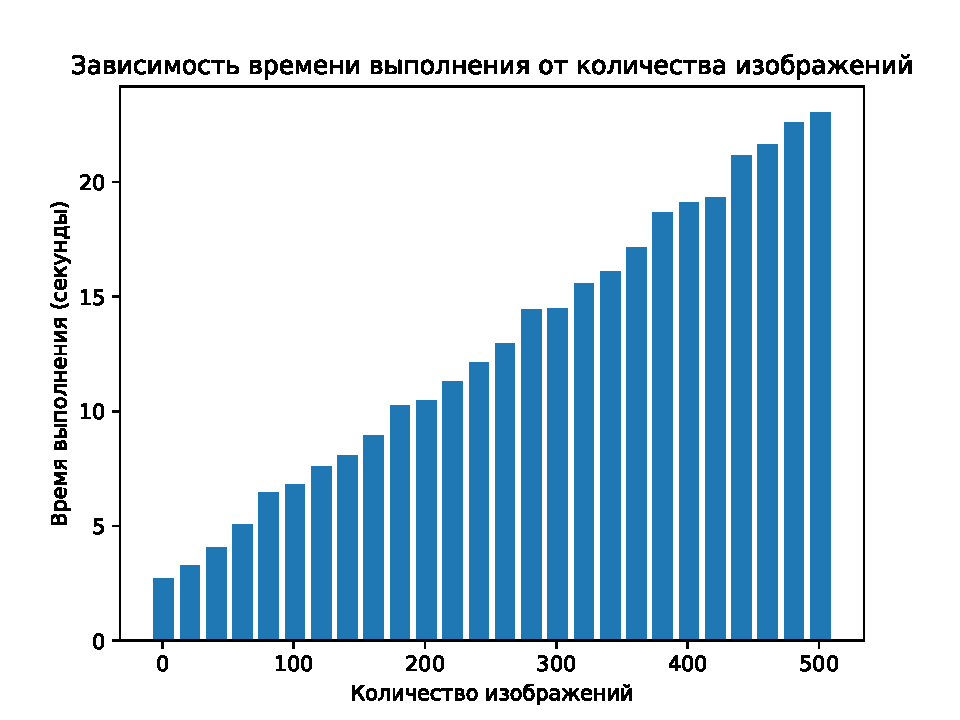
\includegraphics[scale=0.8]{img/count_time_bench.pdf}
	\caption{Зависимость времени работы метода от количества изображений}
	\label{fig:count_time_bench}
\end{figure}

\subsection{Сравнение точности модели нейронной сети на изображениях разного размера}
Так как модель нейронной сети требует, чтобы на вход подавались изображения размером 224x224, то есть все изображения большего размера сжимаются до этого размера. Следовательно имеет смысл рассмотреть изображения меньшего размера и сравнить точность.
 
Для сравнения были взяты 100 изображений из валидационного набора данных предварительно приведенных к нужным размерам.

На рисунке \ref{fig:sizes_acc_bench} приведен график зависимости точности модели от размера изображений.
\begin{figure}[H]
	\centering
	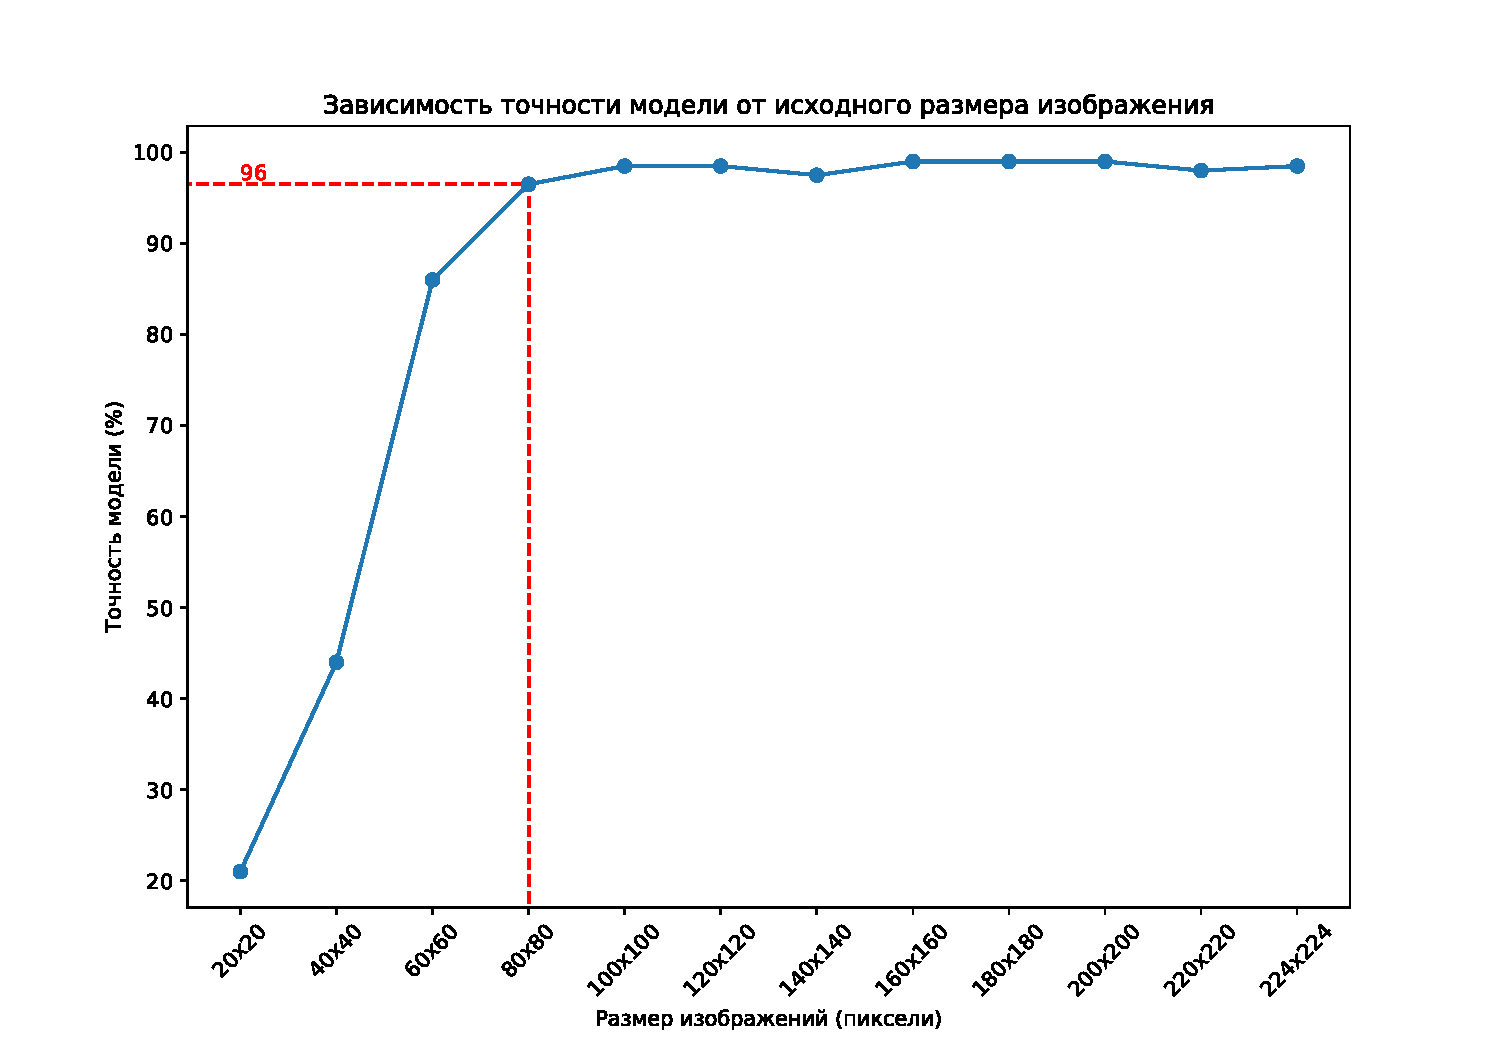
\includegraphics[scale=0.6]{img/sizes_acc_bench.pdf}
	\caption{Зависимость точности модели от размера изображений}
	\label{fig:sizes_acc_bench}
\end{figure}

Из приведенного графика можно сделать вывод, что на изображениях, размер которых меньше 80x80, точность значительно ниже (~85\% для размера 60x60, ~45\% для размера 40x40, ~20\% для размера 20x20), нежели на изображениях большего размера. Из этого следует, что для высокой точности модели и, соответственно, корректной оценки, оптимальным размером изображений является 80x80 и больше.

\newpage
\subsection{Результаты исследования}
На основе сравнений можно сделать следующие выводы:
\begin{itemize}[leftmargin=1.6\parindent]
	\item[--] зависимость времени работы метода от количества изображений линейно;
	\item[--] на обработку, например, 12 часового видео потребуется примерно 36 минут, такое время работы может являться проблемой, если требуется оценивать большое количество водителей;
	\item[--] наиболее оптимальным размером изображений является 80x80 и выше, при размере 80x80 точность модели остается высокой (более 95\%), что позволят хранить меньший объем данных на диске без потери точности.
\end{itemize}


\pagebreak